\newpage
\chapter{Reducing the Design Space}
\label{ch-DS}

Before applying the tools to specified designs, it is helpful to remove as many infeasible options as possible. Due to the complex nature of this problem, all reductions help to make it possible to reach a conclusion in the time available. The reduced design space for the vehicle and the system is summarised in the design option trees, shown in REFERENCE TO DOTs. in this chapter the design reduction decisions are explained.

\section{Vehicle Design Options}
For the design of the propulsion subsystem, options that are not feasible for the scale an urban mobility vehicle are omitted. Therefore turbojet, ramjet and rocket forms of propulsion are crossed out, leaving electric jet propulsion as the only viable option for mass expulsion. Ground assisted propulsion is omitted due to it not being done before. For differential air pressure propulsion, flapped wing options are omitted as they fail to be analysed, due to lack of development. For rotary wing configurations, all rotors and fans are kept as viable design options. For helicopter configuration rotor options, only the coaxial configuration is kept. Tip-jet rotors are non-feasible mainly due to noise, standard rotor configurations have high safety risk due to vortex ring state and are very noisy, tandem configurations require very large blades, and gyro copters do not allow for vertical take off and landing. 

In terms of power source design options, all fuel options are omitted. Nuclear due to safety, carbon based due to sustainability requirements, and hydrogen due to lack of infrastructure to provide a scalable system. This leaves the battery options, for which swappable are omitted due to available fast charging options available. For chargeable battery options, photovoltaics are omitted due to very large surface needed, and induction methods are omitted due to lack of efficiency.

Payload configuration options that are omitted are open and semi- open cabin due to passenger comfort and safety. Due to safety, standing and hanging passenger configurations are excluded.

For control options, options that are disregarded are rocket thrusters, due to lack of practicality. Other options omitted are wing deformations due to lack of existing technology. Gimbal control options are also omitted as they are typically too large. 

\section{System Design Options}
While developing the concepts and comparing their performance in terms of maximum throughput per gate, some trends became quickly obvious. In the case of the centralised system and the pure on-demand system, the vehicles must make multiple takeoff and landing cycles before they can charge. In the cases where the cruise altitude is low, and/or the ratio of energy required for takeoff and ascent ($E_\text{TO} ratio$) is lower than 20\%, these options are more feasible. The main advantage being increased customer choice. However, even with a moderate cruise altitude, the $E_\text{TO}$ was over 40\%.

The result is that most of the concepts were unable to takeoff and ascend to cruise altitude more than once per charge and cover any significant distance. Concepts that could, had a very limited range, and required large rotors or incredibly high energy density batteries.

In addition, making single ascent trips between charges is much more energy efficient, and therefor cheaper, resulting in lower ticket costs. For these reasons, only the port-to-port system was considered in the evaluation and final trade-off.

\begin{wrapfigure}[18]{r}{0.35\textwidth}
    \centering
    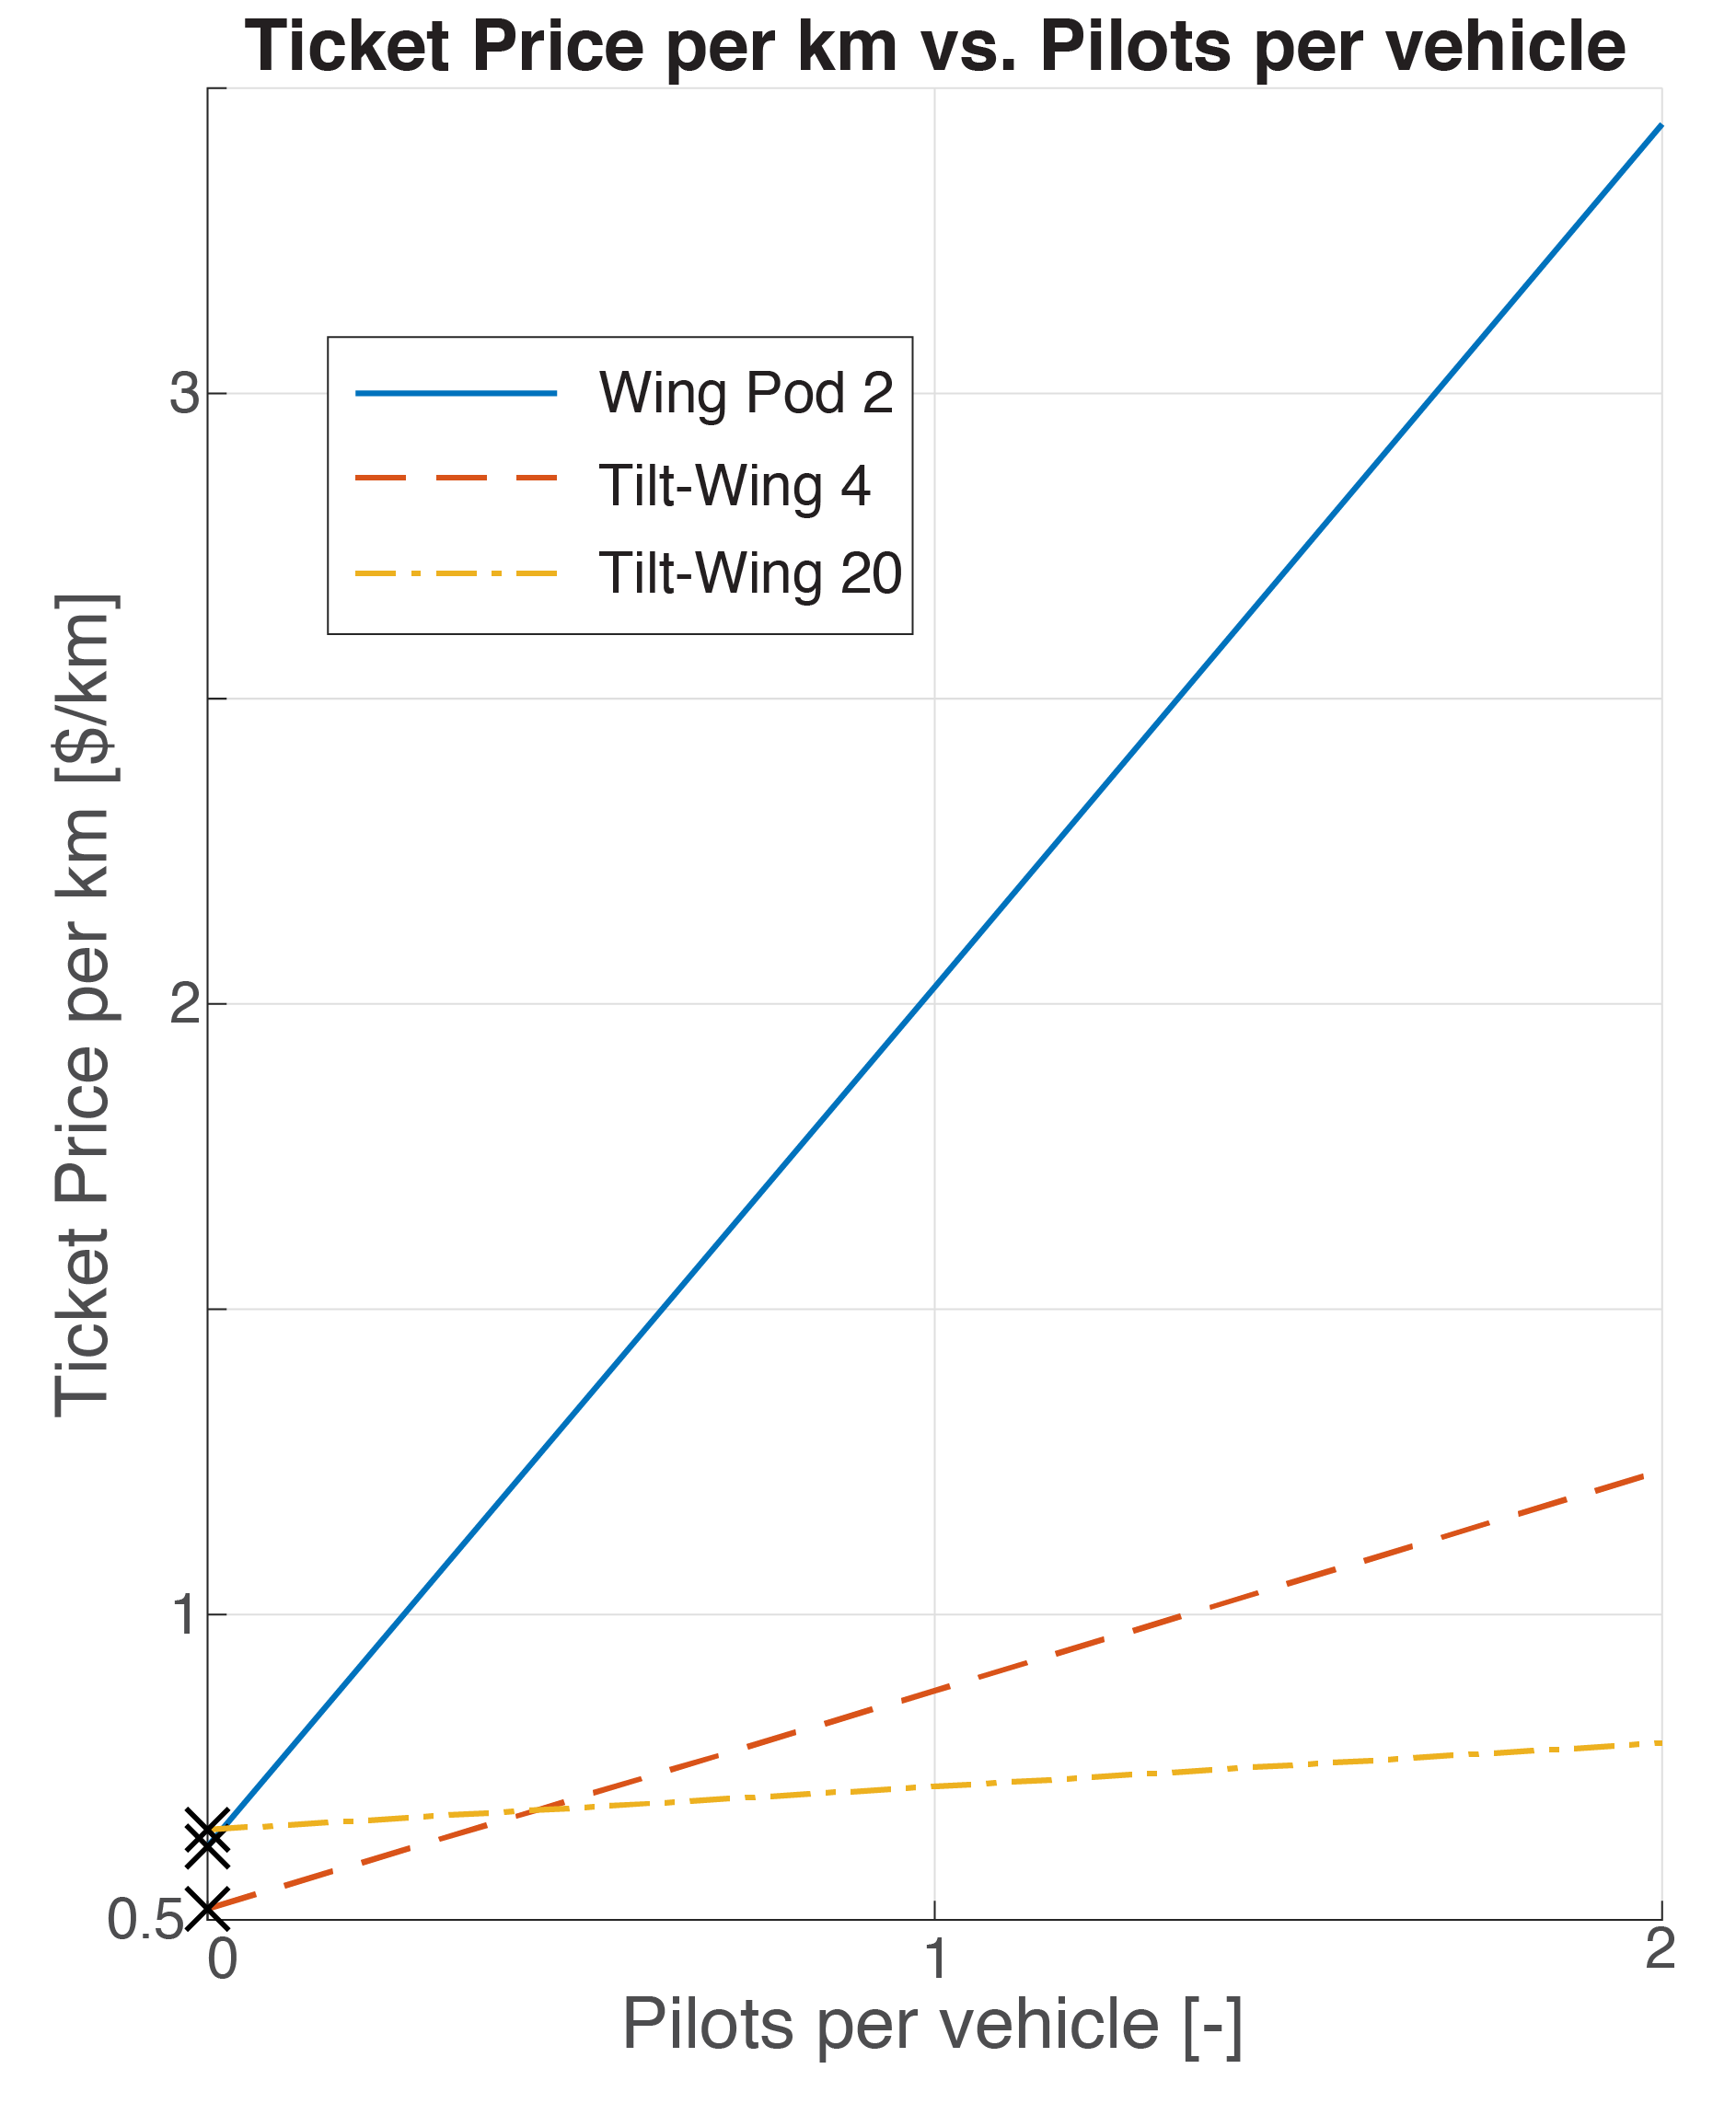
\includegraphics[width=0.35\textwidth]{Figures/Pilots_TPrice_perkm.png}
    \caption{Ticket price increases rapidly if pilots are carried on board.}
    \label{fig:pilotedcost}
\end{wrapfigure}

Additional design options were removed due to related reasons. For example, if all flights are port-to-port, then landing in ground clearings would only occur in emergency situations. A mobile charging recovery unit would be required, but would not be part of normal operations. Landing in ground clearings on regular basis also introduces safety concerns, as securing the site is more difficult.

Battery swapping is not considered either, since it was determined from available battery technology that fast-charging during boarding is very feasible. Designing for batteries that can be quickly swapped also requires increased mass.

Different launch assist ideas were quickly dismissed as few are developed or safe for use.

Using the tools, for all concepts, carrying a pilot on-board become prohibitively expensive. \autoref{fig:pilotedcost} shows how the ticket price per km increases when adding pilots, especially for the smaller vehicles. With the availability of autonomous control becoming more likely in the near future, this technology is considered to be a driving requirement. Having pilots on-board, effectively kills the feasibility of an affordable air taxi service. During the trade-off, it will be considered weather the vehicles require a remote pilot for assistance in certain flight situations, and how many vehicles a single pilot can monitor at once.



\section{Battery Selection}
 From the vehicle design option tree it was determined to use battery electric propulsion for all concepts entering the trade off. It is therefore a crucial step of the concept definition stage to determine the specific battery properties for each vehicle being conceptualised. The reason for this is because the specific battery properties are imperative to the sizing and performance characteristics that allow the tools to evaluate the concepts. A battery database was therefore made to evaluate existing batteries and their characteristics.

 \subsection{Battery Database}
 A battery database listing 26 existing batteries and their respective characteristics as per May 2018 was therefore put together. The database is shown in \autoref{ap:Celldatabase}. During the vehicle definition phase, a selection of the battery is made by evaluating the technical requirements of the vehicle concept against the key characteristics of the battery. The key characteristics include power density, energy density, cost and maximum charge rate. 
 \paragraph{Power Density} Power density was computed by dividing the power output of the cell by its mass. This allows for the capability of a unit mass of the battery to satisfy the power requirement to be evaluated. This then gives information whether for a given vehicle concept the MTOW and power output diverge for a given battery selection. This then gives an indication of whether the altering is needed in the total power output or battery selection. 
 \paragraph{Energy Density}  The energy density is found via the product of nominal capacity and cell voltage, giving the total energy capacity of the cell. The energy density gives an indication of whether the range requirements can be satisfied, and whether for a given concept the MTOW and energy required diverge.
 \paragraph{Battery Cost} The cost was measured by finding the cost of the cell in US dollars and was normalised by dividing by the cell mass. This allows the cost tool to compute the energy cost as an input to the function for average ticket price. For some batteries, it was not possible to access the price of the cell, for example for the Kokam UAV battery series. In order to find the cost per unit mass for these cells, a linear interpolation was performed against the sum of power and energy densities. 
 \paragraph{Charge Rate} The charge c-rate was found, and was multiplied by the total energy and divided by the mass of the cell. This allowed a measure of the amount of energy being charged per unit time and mass to be found. This is a direct input to find charge time for a given concept, which in turn allows the maximum throughput to be found.  

 The main limitation to the database is that the cell models will almost certainly be outdated by the year 2050. It is therefore possible that during the vehicle concept definition phase, in order to satisfy performance requirements, selected battery parameters are overestimated from their actual values given in the database. What the database is still useful in showing is that there is a trade off between the different technical performance of given cell. For example high energy density often is shown to imply a relatively low power density, and a high charge c-rate correlates to a lower energy density. The database allows these correlations to be correctly be taken into account during the selection of battery properties of the vehicle. 
 
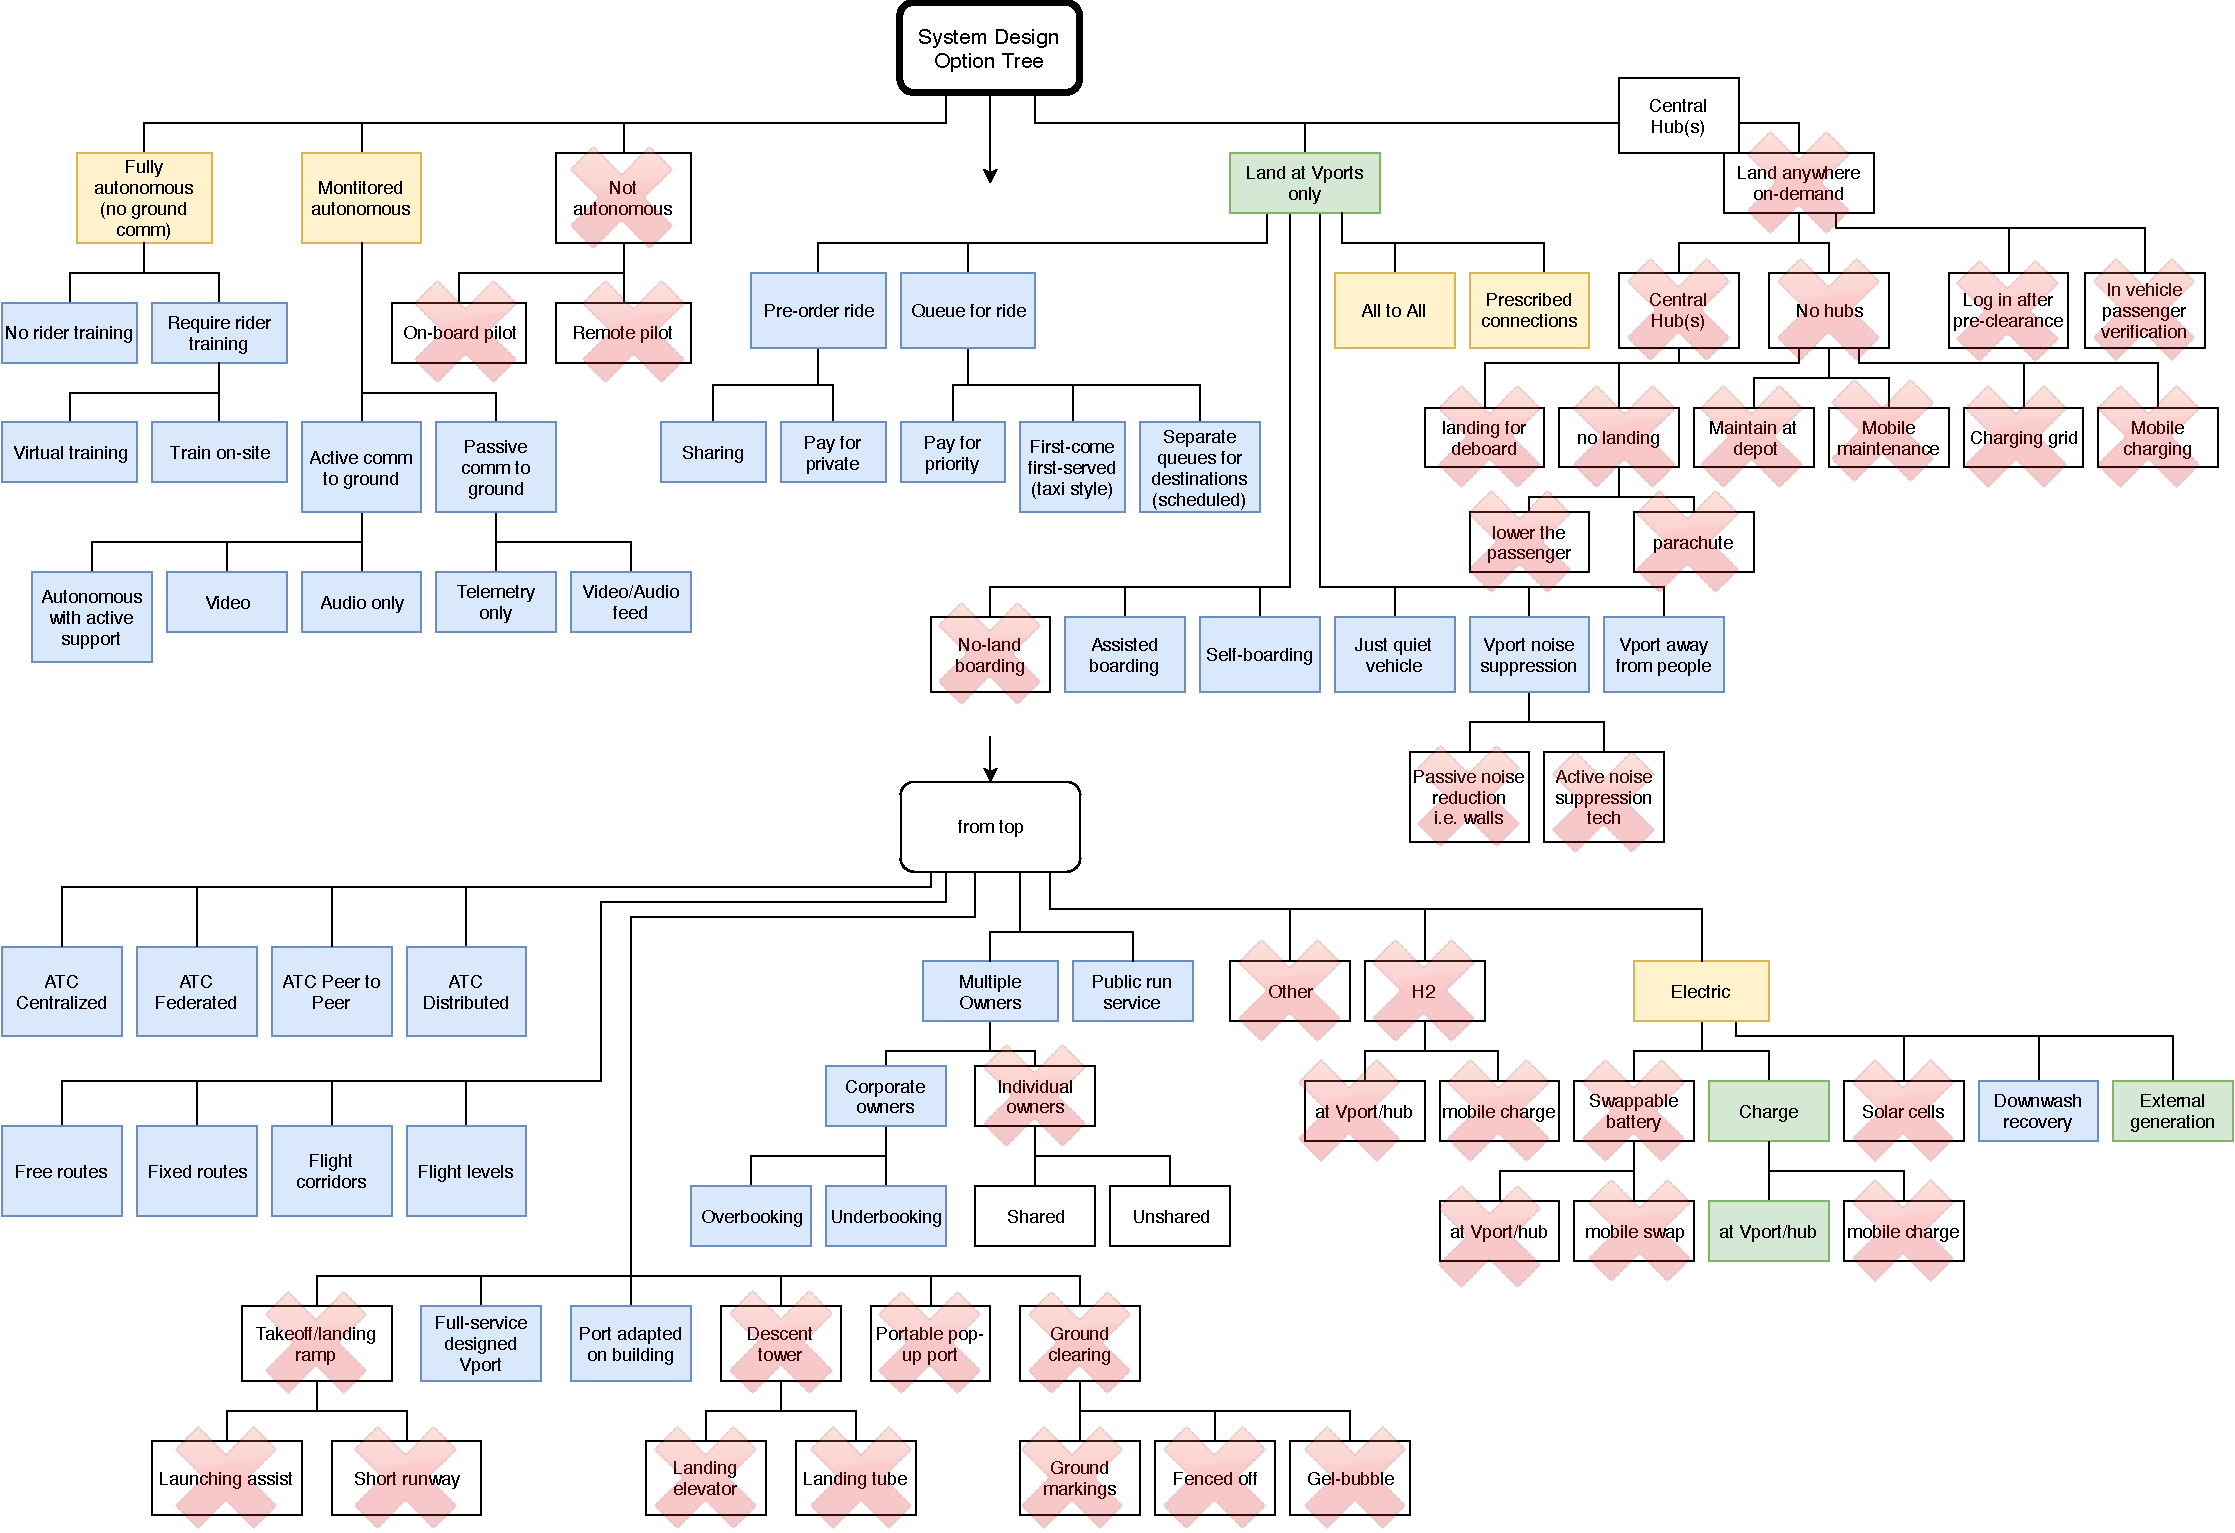
\includepdf[pages={1},fitpaper,pagecommand={\thispagestyle{plain}}]{Figures/Baseline-DOTsystem.pdf}
 
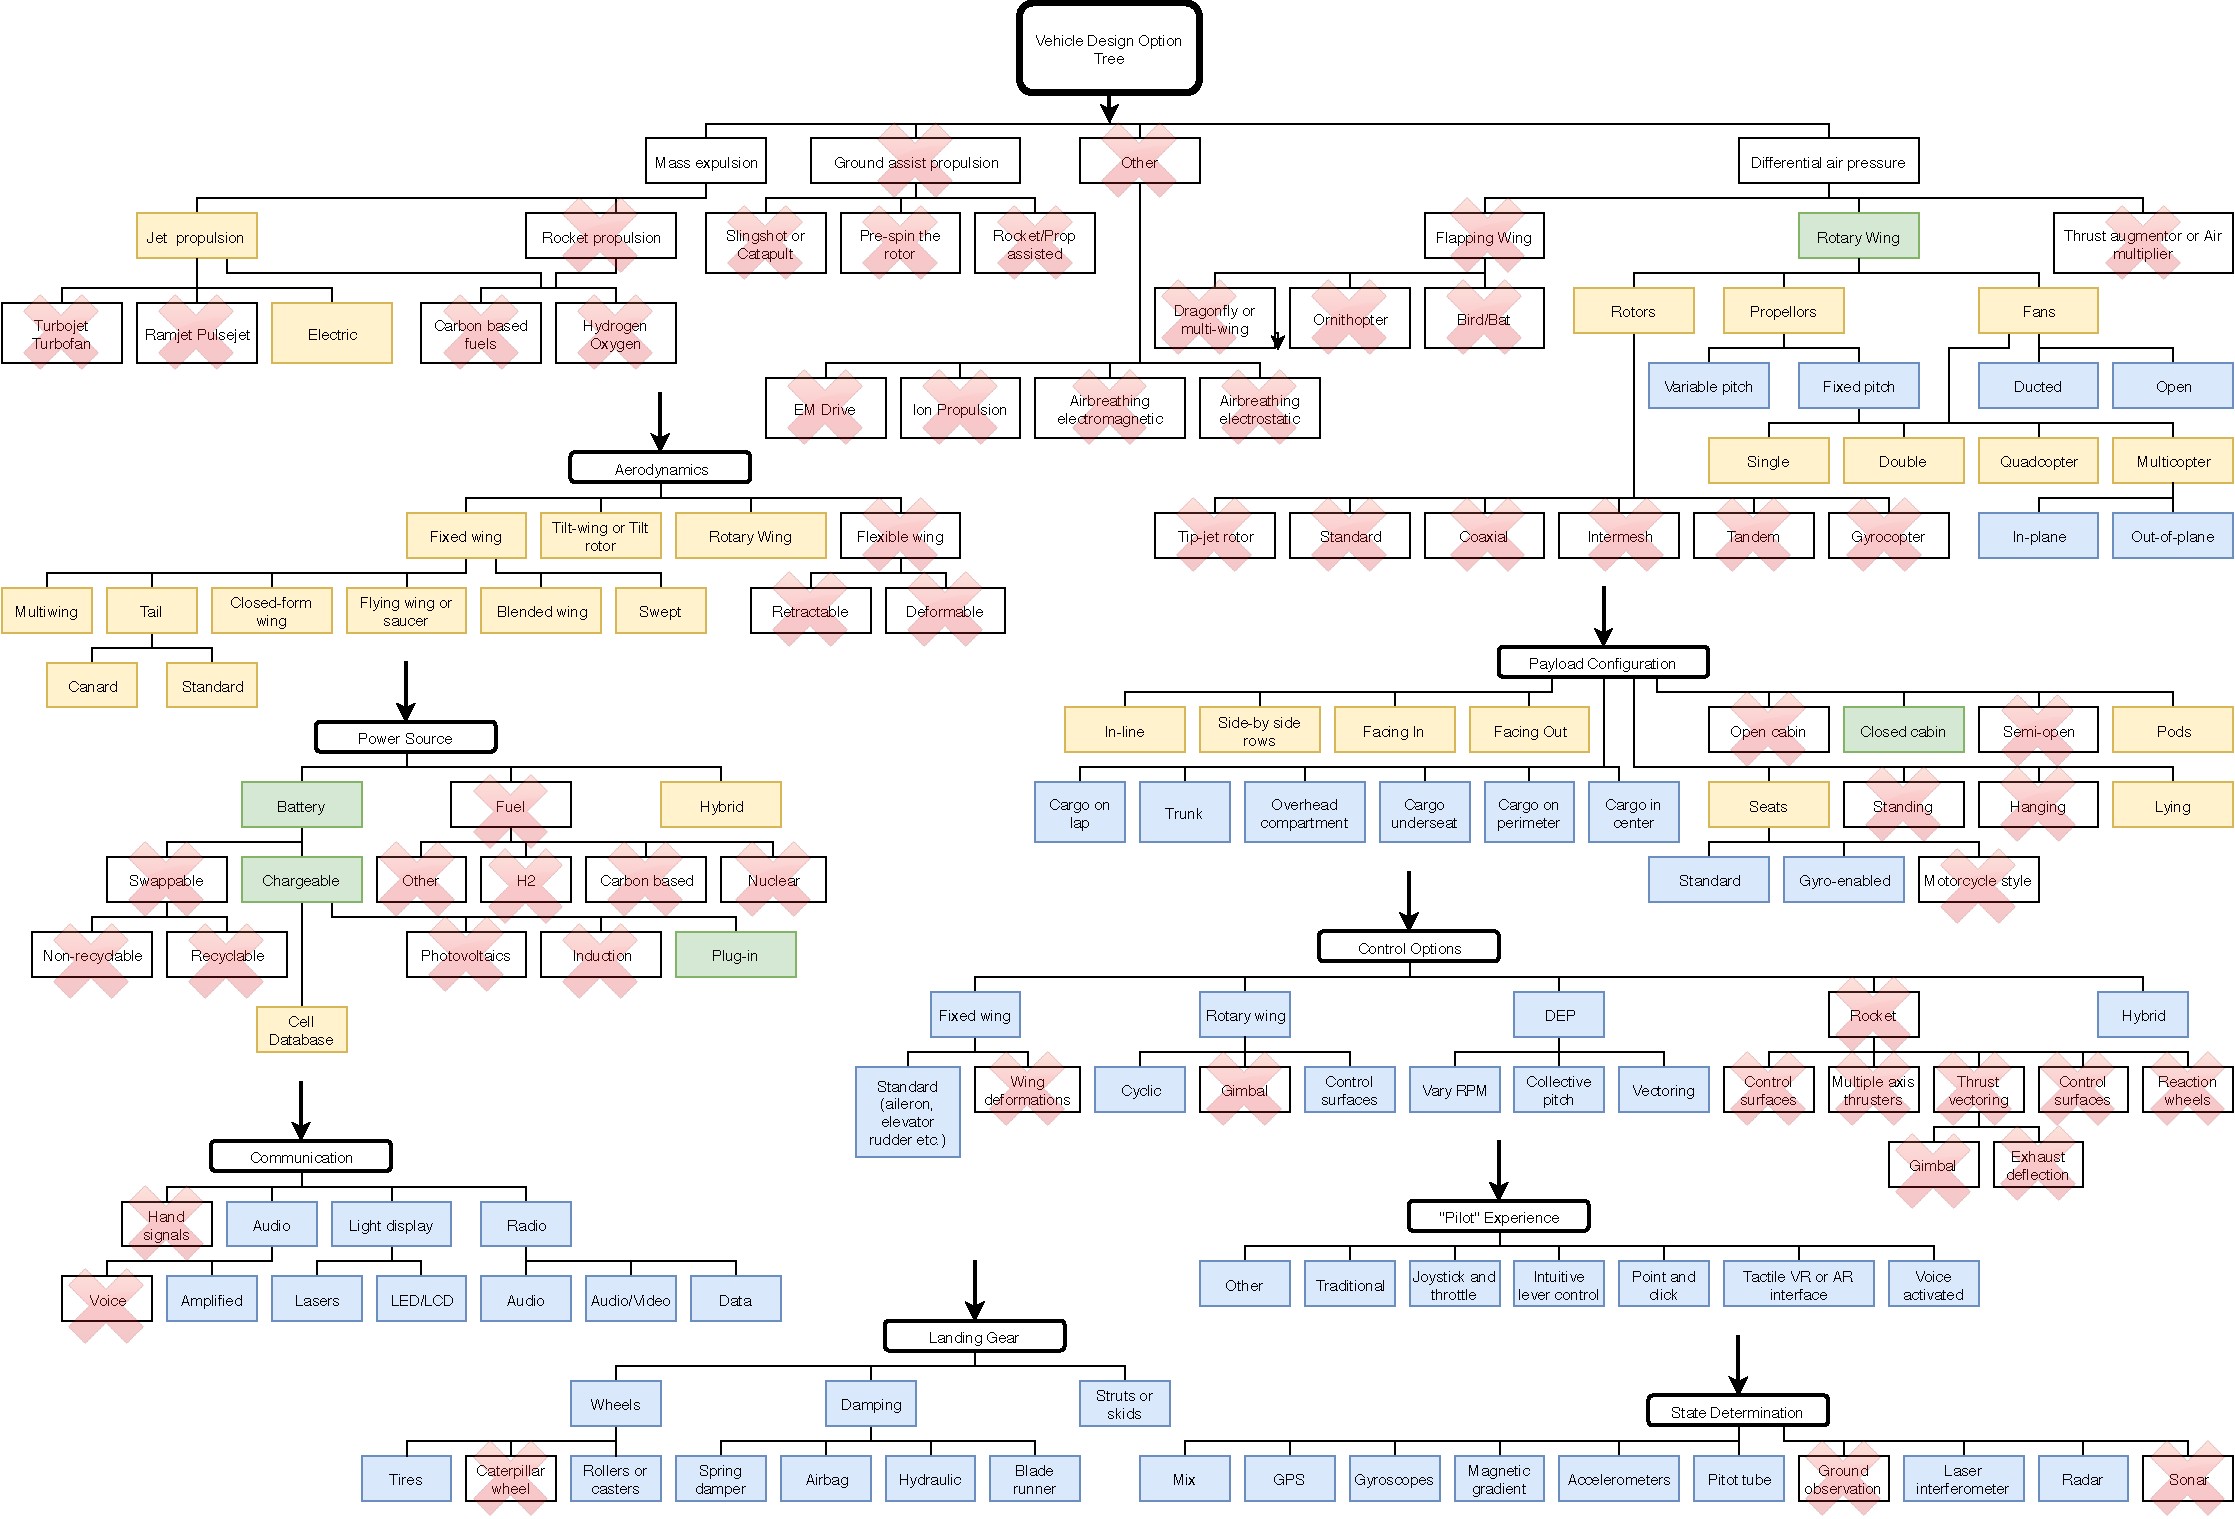
\includepdf[pages={1},fitpaper,pagecommand={\thispagestyle{plain}}]{Figures/Baseline-DOTvehicle.pdf}